\section{Geforderte Funktionseigenschaften}
Die zu schreibende MATLAB Funktion soll nach Fertigstellung in weiteren MATLAB Programmen zum Einsatz kommen. Daher ist es wichtig, dass sämtliche Daten die für das Ausführen erforderlich sind bereits im Code vorliegen und nicht importiert werden müssen. Es sollen auch sonst nach dem Ausführen keine weiteren Maßnahmen oder Eingaben getätigt werden müssen. Um diesen Voraussetzungen gerecht zu werden, ist es erforderlich vor allem große Datensätze im Code einzubinden.\label{createstruct} Bei dieser Arbeit ist das zum einen die Städteliste mit ihren über 1000 Einträgen und zum anderen das Verzeichnis mit allen Registeradressen, in Summe über 340 Positionen. Daneben gibt es noch ein paar weitere Eigenschaften, die an dieser Stelle kurz aufgeführt werden.
\begin{itemize}
\item wiederholte Ausführung des Datenabrufs in bestimmten Zeitabschnitten ohne dabei MATLAB komplett zu blockieren
\item Handhabung der kompletten MODBUS Kommunikation, insbesondere des Datenabrufs, der -verarbeitung und der Parametersetzung
\item Interpolation der ausgelesenen Werte, um unterschiedliche zeitliche Auflösungen zu erhalten
\item Datensicherung derart, dass jeder Datenabruf in einer eigenen Datei und die Summe aller abgerufenen Werte in einer anderen Datei gespeichert werden
\item Fehlervermeidung bei der Eingabe von Inputparametern
\item Aufbau und Beendigung der seriellen Schnittstelle mit der Wetterstation
\item einfache und kurze Inputparameter
\end{itemize}
Nachdem die Eigenschaften nun bekannt sind, soll in den nachfolgenden Unterkapiteln die genaue Umsetzung im Programmcode erläutert werden. Hierzu wird zunächst eine grobe Struktur des Programmaufbaus in Abbildung \textbf{\ref{fig:flowchart}} gegeben. 
\begin{figure}
\centering
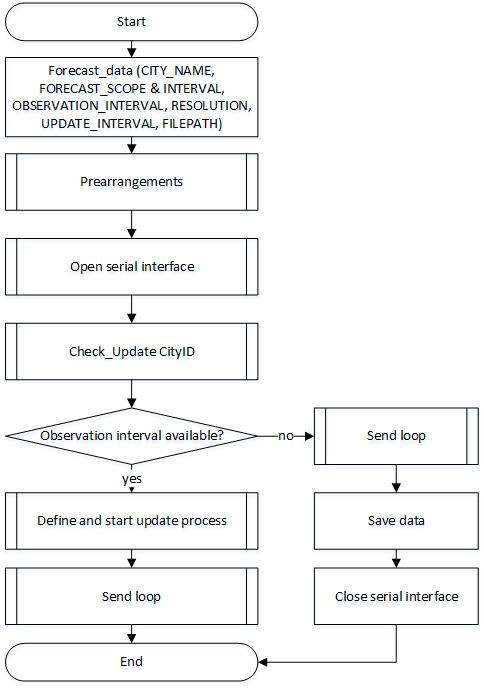
\includegraphics[scale=1]{programm/flowchart}
\caption{Ablaufplan der Funktion forecast\_data}
\label{fig:flowchart}
\end{figure} 
Wie in der Abbildung \ref{fig:funkaufruf} zu erkennen, ist es möglich für die Funktion \textsf{forecast\_data} sieben Eingabeparameter zu definieren. 
\begin{enumerate}
\item Wetterregion
\item Prognosebereichsdefinition
\item Start des Beobachtungszeitraums
\item Ende des Beobachtungszeitraums
\item zeitliche Auflösung
\item Updateintervall
\item Pfadangabe des Speicherortes (optional)
\end{enumerate}
\begin{figure}
\centering
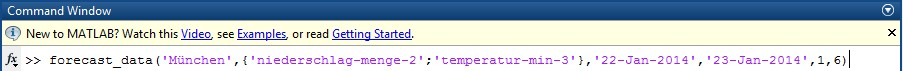
\includegraphics[scale=0.7]{programm/funkaufruf}
\caption{Beispiel für den Funktionsaufruf}
\label{fig:funkaufruf}
\end{figure}
Die Wetterregion wird als Stadtname in Stringformat übergeben. Die Prognosebereichsdefinition besteht aus drei Teilen, die als String in diesem Format 'Prognosebereich-Prognosedetail-Prognoseintervall' aufgebaut ist. Der erste Teil gibt den Wetterbereich an. Hier stehen alle Einträge in der Spalte Prognosebereich der Tabelle \ref{tab:detaildatenstruktur} im Anhang zur Verfügung. Die Prognosedetaildaten können der zweiten Spalte dieser Tabelle entnommen werden. Der dritte Parameter gibt die Anzahl der auszuwertenden Tage an, dabei steht der Wert 1 für den aktuellen Tag ohne Prognose und die Werte 2, 3, 4 für eine entsprechende Erweiterung des aktuellen Tages um die Prognosetage 1, 2 und 3 sofern vorhanden. Um mehrere selektive Prognosebereiche abzurufen, gibt es die Möglichkeit diese als Cell-Array zu definieren. Dabei wird das Cell-Array als Zeilenvektor in dieser Form {Prognosebereichsdefinition\_1;Prognosebereichsdefiniton\_2} definiert. Möchte man keine gesonderte Auswahl treffen und einfach alle möglichen Wetterdaten abrufen, so kann hier an dieser Stelle der Input 'all' erfolgen. Der Beobachtungszeitraum wird durch zwei Daten begrenzt, die ebenfalls als String in dieser Formation 'dd-mmm-yyyy', wobei mit mmm der englische Monatsname gemeint ist, angegeben werden. Die zeitliche Auflösung wird als Double eingetragen. Hier sind die Werte 1, 0.5, 0.25, 0.08 stellvertretend stehend für 1 Stunde, eine halbe Stunde, eine viertel Stunde und 5 Min., möglich. Soll keine Interpolation der Daten erfolgen, so trägt man hier den Wert 6 ein. Das Updateintervall wird ebenfalls als Double definiert. Hier stehen die Werte 6, 12, 24 zur Verfügung, welches einem vier-, zwei- und einmaligen Update am Tag entspricht. Die Pfadangabe wird wiederum als String eingegeben. Die Abbildung \ref{fig:funkaufruf} gibt hierzu ein Beispiel. Es wird für die Region München die Niederschlagsmenge für den heutigen und ersten Folgetag, die minimale Temperatur für den heutigen und die beiden nachfolgenden Tage, über einen Zeitraum von zwei Tagen abgerufen. Dabei beträgt die zeitliche Auflösung 1 Stunde und das Intervall in denen Updates gestartet werden 6 Stunden. Nachdem hier kein Speicherpfad angegeben ist, wird ein Ordner mit der Bezeichnung \enquote{Aufzeichnungen} im aktuellen MATLAB Ordner erstellt und als Speicherort ausgewählt. 
\section{Vorbereitende Maßnahmen}
\subsection{Zuweisung variabler Inputparameter und Variableninitiierung}
Als erstes wird der Default-Ordner \textit{default\_filepath} für das Abspeichern der Daten festgelegt. Dabei wird nachgesehen, ob lediglich eine Laufwerksangabe vorliegt oder nicht. Für den Fall, dass variable Inputparameter übergeben wurden, wird zuerst geprüft, ob die Anzahl der geforderten Werte vorhanden ist. Ist das nicht der Fall, so wird eine Meldung an den Nutzer ausgeben und die Funktion beendet. Stimmt die Anzahl, werden die Werte Funktionsvariablen zugeordent. Möchte man den Zeitpunkt zu dem der erste Datenabruf nach Ausführen der Funktion erfolgt verschieben, so kann man einen zeitlichen Offset als 7tes Inputargument übergeben. Wenn Startzeitpunkt des Beobachtungsintervalls und Funktionsausführung am gleichen Tag liegen, so bewirkt der Offset eine Verschiebung vom Ausführungszeitpunkt der Funktion an. Liegt das Startdatum jedoch in der Zukunft, so findet die Verschiebung von 0.00 Uhr des Startdatum an statt. Ist zudem noch eine Pfadangabe zu einem Speicherort der Funktion übergeben worden, so wird diese ebenfalls einer Funktionsvariablen zugewiesen. Wurden keine Angaben zu den beiden Werten gemacht, so wird im aktuellen MATLAB Ordner der Default-Ordner \enquote{Aufzeichnungen} als Speicherplatz definiert und der Offset auf Null gesetzt. Existiert der Ordner bereits, erfolgt eine Meldung auf deutsch. Wurden keine variablen Parameter übergeben (entspricht einem einmaligen sofortigen Abruf), so wird die zeitliche Auflösung auf 1 Stunde festgesetzt und ebenfalls der Default-Speicherort vorgegeben. 
\lstinputlisting[firstline=69, lastline=108]{programm/forecastdata.m}
Nachdem die \textit{forecast\_defintion} sowohl als String als auch als Cell-Array übergeben wird, im späteren Programmablauf aber nur ein Cell-Array erwartet wird, muss noch eine Konvertierung stattfinden.\label{sendloop} Mit dem ersten Funktionsaufruf, an dem noch kein Tageswechsel auftreten kann, werden die Variablen \textit{daychange\_flag} und \textit{daychange\_counter} auf Null gesetzt und dem Base-Workspace zugewiesen. Ebenso initialisiert werden die späteren Datencontainer \textit{weather\_data} und \textit{new\_data}. Wie in Tabelle \ref{tab:parabel} gezeigt, lautet die Slave-ID der Wetterstation \enquote{03}. Diese wird hier der \textit{device\_id} zugeordnet. 
\lstinputlisting[firstline=110, lastline=127]{programm/forecastdata.m}   
\subsection{Aufbau von Strukturen}
\lstinputlisting[firstline=128, lastline=141]{programm/forecastdata.m} 
Wie bereits im vorigen Kapitel~\ref{createstruct} angekündigt, müssen große Datensätze in Strukturen gepackt werden um später aus ihnen Daten zu gewinnen. Sollen alle Wetterdaten abgerufen werden, ist es erforderlich ein Cell-Array aufzubauen, welches alle Wetterdatenanfragen beinhaltet. Danach werden Strukturen angelegt, die die Registeradressen und Städtenamen abbilden. Die letzten beiden Strukturen müssen wieder im Base-Workspace verfügbar sein da andere Funktionen auf sie zurückgreifen werden.
\subsection{Überprüfung der Eingabeparameter}
\lstinputlisting[firstline=145, lastline=169]{programm/forecastdata.m}
Diese for-Schleife bearbeitet alle übergebenen Wetterdatenanfragen, prüft sie auf Gültigkeit und erstellt zugleich die entsprechenden Datencontainer. Die Datencontainer werden im Base-Workspace eingetragen. Sind ein oder mehrere Eingabeparameter falsch, werden diese dem Nutzer mit einer Nachricht angezeigt und die Funktion beendet.
\lstinputlisting[firstline=1, lastline=1]{programm/inputcheck.m}
Die Funktion \textsf{input\_check} liefert als Outputparameter einen Vektor der angibt, welche Parameter gültig sind. Zusätzlich werden die generierten Fehlermeldungen, die ID der Wetterregion, der Breitengrad und Längengrad ausgegeben. 
\lstinputlisting[firstline=4, lastline=16]{programm/inputcheck.m}
Im ersten Abschnitt des Input Checks wird die Funktion \textsf{get\_city\_id} aufgerufen, um die ID der Wetterregion, den Längen- und Breitengrad zu ermitteln. Ist die ID nicht in der Liste zu finden, wird die entsprechende Vektorposition \textit{val\_inpt} auf false gesetzt.  
\lstinputlisting[firstline=1, lastline=18]{programm/getcityid.m}
In dieser Funktion muss zuerst die im Base-Workspace befindliche Variable \textit{city\_list} zugänglich gemacht werden. Danach wird die Spalte mit den Städtenamen mit \textsf{nominal} konvertiert, um im darauffolgenden Schritt eine einfache Suche der Position in der Liste zu starten, die dem Städtenamen entspricht. In der Variable \textit{city\_data\_set} sind nun alle Werte dieser Liste, die der Position entsprechen, enthalten. Eine einfache Wenn-Dann-Bedingung weist die Daten den Outputparametern zu.   
\lstinputlisting[firstline=19, lastline=62]{programm/inputcheck.m}
An dieser Stelle wird die Wetterdatenanfrage analysiert. Kommt in dem Ausdruck nicht zweimal ein Querstrich vor, ist die Eingabe schon fehlerhaft. Wenn doch, werden die drei einzelnen Bestandteile mit Listen abgeglichen und bei entsprechender Existenz keine Fehlermeldung ausgegeben.  
\lstinputlisting[firstline=65, lastline=103]{programm/inputcheck.m}
Die Überprüfung des Observationszeitraums erfolgt dahingehen, dass der Ausdruck ein Datumsformat darstellen muss, den MATLAB mittels \textsf{datenum} konvertieren kann. Ist dies nicht möglich, liegt ein Fehler vor. Sind die Datumsformate korrekt, so kann es immer noch der Fall sein, dass das Startdatum in der Vergangenheit oder vor dem Enddatum liegt. Auch hier werden entsprechende Fehlermeldungen generiert.
\lstinputlisting[firstline=105, lastline=132]{programm/inputcheck.m}
Im letzten Teil der Überprüfung werden die Werte der zeitlichen Auflösung und des Updateintervalls wieder mit Listen abgeglichen. Ist der Gültigkeitsvektor in der boolschen Überprüfung wahr, werden keine Fehlermeldungen ausgegeben. Andernfalls wenn weniger als 10 Fehlermeldungen angefallen sind, muss der letzte Vektoreintrag der Fehlermeldungen leer sein. Dies ist erforderlich, um den nachfolgenden Print-Befehl ausführen zu können. 
\subsection{Verfügbarkeitsprüfung der seriellen Schnittstelle}   
\lstinputlisting[firstline=173, lastline=189]{programm/forecastdata.m} 
Existiert bereits eine Variable \textit{serial\_interface} im Base-Workspace, so wird diese gelöscht. Zudem werden alle anderen seriellen Schnittstellen gelöscht um zu vermeiden, dass bereits eine andere serielle Schnittstelle den COM6 Port belegt hat. Danach wird die Verfügbarkeit des COM6 Ports festgestellt. Ist dies nicht der Fall, wird eine Fehlermeldung an den Nutzer ausgegeben und die Funktion beendet.
\section{Aufbau der seriellen Schnittstelle}
\lstinputlisting[firstline=191, lastline=192]{programm/forecastdata.m}
Die Funktion \textsf{open\_serial\_port} enthält bereits alle in der Tabelle \ref{tab:parabel} auf Seite~\pageref{coilabfrage} festgelegten Schnittstellenparameter.
\lstinputlisting[firstline=1, lastline=17]{programm/openserialport.m}
MATLAB bietet für den Aufbau einer seriellen Schnittstelle eine Funktion namens \textsf{serial} an. Diese wird hier zur Erstellung der Variable \textit{serial\_interface} angewandt. Die Variable wird dem Base-Workspace zugewiesen und die serielle Schnittstelle mit dem Befehl \textsf{fopen} geöffnet. Der Nutzer wird über den Schnittstellenaufbau informiert.
\section{Abgleich der Wetterregion im Register}
\lstinputlisting[firstline=195, lastline=221]{programm/forecastdata.m}
Da der Wechsel einer Wetterregion unter Umständen bis zu drei Tagen dauern kann, bis alle anliegenden Werte Gültigkeit besitzen, wird in diesem Teil des Codes zuerst die bereits eingetragene Stadt-ID ausgelesen und mit der in dem Funktionsaufruf Angegebenen verglichen. Weichen die beiden Werte voneinander ab, so wird der Nutzer per Tastatureingabe aufgefordert dem Wetterregionenwechsel zuzustimmen. Er hat somit die Gelegenheit einen versehentlichen Wechsel abzubrechen. Anschließend wird der neue Wert im Register eingetragen. 
\section{Festlegung der Timerparameter und Starten des Timers}
\lstinputlisting[firstline=226, lastline=263]{programm/forecastdata.m}
Um die Eigenschaft des wiederholten Datenabrufs zu implementieren wurde das Timer-Objekt von MATLAB implementiert. Es bietet den Vorteil im Hintergrund zu laufen ohne dabei MATLAB komplett zu blockieren. Für die Initialisierung dieses Objekts müssen zuerst ein paar Parameter ermittelt werden. Insbesondere betrifft dies das Timerintervall, die Anzahl der Timerausführungen und die Timerverzögerung. Das Timerintervall lässt sich einfach dadurch berechnen indem die Variable \textit{update\_interval} mit der Anzahl an Sekunden für eine Stunde multipliziert wird. Die Anzahl der Timerausführungen ergibt sich dann durch die zur Verfügung stehenden Stunden im Beobachtungszeitraum dividiert durch die Länge des Timerintervalls. Liegt der Beobachtungszeitraum in der Zukunft, so muss die Timerverzögerung genau die Länge vom Funktionsaufruf bis zum Startdatum aufweisen. Bei der Berechnung dieser Angaben sind die MATLAB Funktionen \textsf{days365}, \textsf{datevec} sowie \textsf{etime} äußerst nützlich.
\lstinputlisting[firstline=270, lastline=282]{programm/forecastdata.m}    
Mit der Zuweisung \enquote{t = timer} wird in der Variablen \textit{t} das Timer-Objekt erzeugt. Die Eigenschaften können dann ähnlich einer Struktur in MATLAB aufgerufen und bestimmt werden. Zu bestimmen sind die Timerverzögerung (\textit{t.StartDelay}), das Timerintervall (\textit{t.Period}), die Timerausführungen (\textit{t.TasksToExecute}), sowie die Ausführungsmethode (\textit{t.ExecutionMode}). Die Ausführungsmethode \enquote{fixedRate} garantiert, dass in genau gleichen Timerintervallen die in der Timerfunktion (\textit{t.TimerFcn}) definierte Funktion ausgeführt wird. Wird der Timer durch einen Fehler oder durch einen Abbruchbefehl unterbrochen, so legt man in der Timerstopfunktion fest, was geschehen soll.
\lstinputlisting[firstline=1, lastline=19]{programm/stoptimer.m}  
Kommt es zu einem Timerabbruch, so wird eine Meldung an den Nutzer ausgegeben, das Timer-Objekt gelöscht und der Datencontainer mit den fortlaufenden Werten abgespeichert. Außerdem wird die serielle Schnittstelle beendet. Der Dateiname für den Datencontainer setzt sich zusammen aus der Wetterregion, der angewandten zeitlichen Auflösung, dem aktuellen Datum und dem aktuellen Datum in Unix Zeitformat.    
\section{Abschicken der MODBUS-Anfragen}
\lstinputlisting[firstline=1, lastline=2]{programm/sendloop.m}
Die Funktion, die das sequentielle Abschicken und Verarbeiten der einzelnen MODBUS Nachrichten übernimmt wird hier erläutert.
\lstinputlisting[firstline=5, lastline=35]{programm/sendloop.m}
Nachdem die Eingabeparameter übergeben wurden, werden die im Base-Workspace vorhandenen Variablen \textit{daychange\_flag}, \textit{daychange\_counter}  sowie der Datencontainer \textit{w\_dat} für die Langzeitarchivierung in dieser Funktion bereitgestellt. Eine for-Schleife durchläuft dann alle Wetterdatenanfragen die in \textit{fc\_def} definiert wurden. Beim ersten Durchlauf muss geprüft werden, ob bereits zu einem früheren Zeitpunkt Daten ausgelesen wurden damit ein Tageswechsel signalisiert werden kann. Hierzu wird der letzte Zeitstempel des letzten Datenabrufs, sofern vorhanden, mit dem aktuellen Datum verglichen. Ist das Ergebnis ungleich Null, liegt ein Tageswechsel vor und die Variablen werden entsprechend angepasst und im Base-Workspace aktualisiert.
\lstinputlisting[firstline=38, lastline=94]{programm/sendloop.m}
Im nächsten Schritt wird das Intervall für die auszulesenden Wetterdaten zusammengestellt. Hierbei muss unterschieden werden zwischen den stündlichen Werten der mittleren Lufttemperatur, dem begrenzten Prognosehorizont von Luftdruck und Solarleistung und den verbleibenden Daten. Gibt der Nutzer eine zu hohe Zahl für Luftdruck oder Solarleistung ein, so wird auf die möglichen Werte angepasst und eine Warnung ausgegeben.
\lstinputlisting[firstline=95, lastline=111]{programm/sendloop.m}
In diesem Abschnitt wird die MODBUS Nachricht erstellt und einer Funktion übergeben, die das Schreiben und Lesen auf der seriellen Schnittstelle übernimmt. Die Startadresse des Registers ergibt sich aus dem Prognosebereich, dem Prognosedetail und dem Anfangszeitpunkt zu dem die Werte ausgelesen werden sollen. Die Endadresse wir im gleichen Verfahren ermittelt. Die Differenz aus den beiden Adressdaten ergibt die Registeranzahl. Gemäß der MODBUS Spezifikation liegen nun alle Daten vor, die zur Kommunikation notwendig sind. Lediglich der Cyclic Redundancy Check fehlt noch. Dieser wird in der Funktion \textsf{gen\_msg} erstellt und der PDU zusammen mit der Slave-ID angeheftet. Wie die momentane Verbindungsqualität zum Zeitpunkt der Anfrage ist, wird kurz darauf abgerufen. Alle für die weitere Verarbeitung erforderlichen Daten werden nun an die Funktion \textsf{send\_and\_receive\_data} übergeben. 
\lstinputlisting[firstline=112, lastline=131]{programm/sendloop.m}
Ist die for-Schleife durchlaufen und alle Daten liegen in den Datencontainern, wird der vollzogene Abruf in dem Container \textit{new\_data} mit entsprechendem Dateinamen abgespeichert. Der Dateiname setzt sich dabei aus dem Pfad zum Speicherort, dem Stadtnamen, der gewünschten Auflösung, dem aktuellen Datum und einem Datum in Unix Zeitformat zusammen. Ist das Speichern abgeschlossen, wird der Datencontainer geleert und neu initialisiert. Der letzte Schritt in diesem Programmteil ist das Update der noch verbleibenden Anzahl an Datenabrufen, welche in der Variable \textit{u\_c\_n} (update cycle number) hinterlegt sind.
\section{Senden und Empfangen}
\lstinputlisting[firstline=1, lastline=31]{programm/sendandreceivedata.m}
In dem Funktionsworkspace der Funktion \textsf{send\_and\_receive\_data} muss die serielle Schnittstelle zugänglich sein. Um die in der Funktion \textsf{send\_loop} generierte Nachricht über die Schnittstelle abschicken zu können, muss sie auf ein geeignetes Format gebracht werden. Dann erst kann die Nachricht mit dem Befehl \textit{fwrite} übermittelt werden. Es wird 1 Sekunde auf die Antwort gewartet. Das bestimmen der empfangenen Bytes und die Angabe beim Lesebefehl \textsf{fread} beschleunigt die Kommunikation enorm. Jetzt liegt die Antwortnachricht des Servers in der Variablen \textit{rx\_data} vor. Die darin enthaltenen Werte wurden als unsigned integer 8 bit empfangen.      
\lstinputlisting[firstline=1, lastline=31]{programm/formatmodbusmsg.m}
Die Funktion \textsf{format\_modbus\_msg} transformiert den String der MODBUS-Nachricht in einen 8-zeiligen Vektor mit dezimalen Werten die den hexadezimalen Werten des Strings entsprechen. 
\section{Rx-Datenverarbeitung}
\lstinputlisting[firstline=1, lastline=7]{programm/rxdataprocessing.m}
Hauptaufgabe der Rx-Datenverarbeitung ist es den empfangenen Funktionscode auszuwerten, die Daten zu isolieren und an eine weitere Funktion zur Bearbeitung zu übergeben. Der rx-Datenstring ist als Zeilenvektor aus einer Reihe von Dezimalzahlen folgendermaßen aufgebaut:
\begin{itemize}
\item an erster Stelle kommt die Slave-ID 
\item an zweiter Stelle folgt der Funktionscode 
\item an dritter Stelle steht die Anzahl der übertragenen Bytes
\item an den darauffolgenden Positionen befinden sich die Datenbytes
\item die beiden letzten Einträge beinhalten den CRC-Wert
\end{itemize}
\lstinputlisting[firstline=9, lastline=36]{programm/rxdataprocessing.m}
Zuerst wird der Funktionscode auf einen Fehlercode hin in der Funktion \textsf{fcod\_check} kontrolliert. Dies ist dann der Fall, wenn er nicht den Wert 1, 3 oder 6 besitzt. Um welchen Ausnahmefall es sich dann handelt, wird in der Switch-Abfrage geklärt und das Programm stoppt mit einem Fehler.  
\lstinputlisting[firstline=1, lastline=15]{programm/fcodecheck.m}
Ist der Funktionscode in Ordnung wird entschieden, wie mit den Datenbytes zu verfahren ist. Eine Switch-Abfrage führt zu den entsprechenden Arbeitsschritten. Für den Fall, dass der Funktionscode den Wert 1 oder 6 aufweist, ist die Bearbeitung recht einfach. Es müssen lediglich ein Datenbyte beim Code 1 und zwei Datenbytes beim Code 6 verarbeitet werden.    
\lstinputlisting[firstline=39, lastline=66]{programm/rxdataprocessing.m}

\section{Datenverarbeitung}
\lstinputlisting[firstline=1, lastline=1]{programm/dataprocessing.m}
Das eigentliche Herzstück dieses Programms ist die Datenverarbeitung die mit der Funktion \textsf{data\_processing} gestartet wird. Die notwendigen Parameter sind die empfangen Datenbytes im \textit{data\_string} hinterlegt, die Definition der Wetterdatenabfrage als \textit{fc\_def}, die zeitliche Auflösung in der Variable \textit{res}, die Verbindungsqualität, übergeben als \textit{con\_qual} und die Längen- und Breitengradangabe in Form von \textit{lng} bzw. \textit{lat}. 
\lstinputlisting[firstline=7, lastline=35]{programm/dataprocessing.m}
Zunächst werden die Variablen aus dem Base-Workspace geladen, mit denen gearbeitet wird. Danach liefert die Funktion \textsf{MESZ\_calc} ein Flag für die Mitteleuropäische Sommerzeit. Im Anschluß werden die Listen für einen späteren Datenabgleich erstellt.        
\lstinputlisting[firstline=37, lastline=47]{programm/dataprocessing.m}
Erfolgt nur eine Abfrage der Kommunikationsparameter oder bestimmter Zustände der Wetterstation, muss nur ein Wert ausgewertet werden. Dies geschieht, wenn die If-Bedingung wahr ist. Da die Daten der seriellen Schnittstelle als unsigned int8 Werte empfangen wurden, werden negative Werte ab der Zahl 32769 dargestellt. Um sie zu erhalten muss der Wertebereich von 2 unsigned Bytes abgezogen werden.  
\lstinputlisting[firstline=49, lastline=80]{programm/dataprocessing.m}
Ist die If-Bedingung falsch, handelt es sich um Wetterdaten. Zunächst werden Variablen initiiert. Dabei ist \textit{i} eine Laufvariable, die die Position angibt zu dem ein Datumswechsel stattgefunden hat. \textit{n\_dat\_r} ist die Vektorposition in dem Datencontainer, der jeden einzelnen Datenabruf speichert. Deshalb ist sie immer auf 1 gesetzt. Da die Ausgangsdaten selbst in einer unterschiedlichen Auflösung gegeben sind, müssen mit der Funktion \textsf{res\_factor} auch zwei separate Faktoren für die spätere Interpolation bestimmt werden. Hat ein Abruf bereit zu einem früheren Zeitpunkt stattgefunden, so wird dieser Abruf-Zeitstempel der Variable \textit{t\_rec} zugewiesen. Er bestimmt sich aus dem letzten aufgezeichneten Wert und dessen Rekordstempel. Anschließend wird die Startvariable \textit{sdindex} der nachfolgenden for-Schleife für die zu bearbeitenden Prognosetage bestimmt. Dabei definiert die Position in der entsprechenden Liste diesen Wert. Der Endwert \textit{edindex} der Schleife wird in gleicher Weise bestimmt.   
\lstinputlisting[firstline=82, lastline=118]{programm/dataprocessing.m}
Lag noch kein vorheriger Datenabruf vor, so starten die Positionsvektoren des Datencontainers, der die Daten des Beobachtungszeitraums speichert, bei 1. Hier werden zwei Variablen \textit{w\_dat\_r} und \textit{w\_dat\_org} benötigt. Während die Erste später mit der interpolierten zeitlichen Auflösung voranschreitet, behält die Zweite die ursprüngliche Schrittweite. Die while-Schleife bestimmt nun die Position bei einem evtl. Datumswechsel. Dazu wird die in der Variable \textit{unix\_t\_strt} gespeicherte Zeitreihe durchlaufen bis das Datum dem aktuellen Datum entspricht. Der Wert wird der Vektorposition übergeben. Abhängig ob es sich um Daten handelt die interpoliert werden, bekommt auch die Vektorposition für die originalen Daten einen Wert zugewiesen. Er errechnet sich entsprechend der Auflösung der Daten für die mittlere Lufttemperatur (24 Werte pro Tag) multipliziert mit der Zahl der bis dato vollzogenen Tageswechseln plus eins.      
\lstinputlisting[firstline=120, lastline=184]{programm/dataprocessing.m}
Handelt es sich um einen längeren Datenstring, so muss dieser durchlaufen werden. Es erfolgt eine Initialisierung dieser Variablen. Danach beginnt die Schleife für den Tagesdurchlauf. Zu Beginn wird je nach Schleifenpostition der Anfangs- und Endwert der Schleife für die Tagessegmente bestimmt. Der hier verwendete Aufbau scheint ein wenig kompliziert zu sein und stammt aus einer Version in der es möglich war völlig willkürliche Intervalle zu bestimmen und nicht nur tagesweise den Abruf zu durchlaufen. Sind Start- und Endwerte für die Tagessegment-Schleife bestimmt, wird im letzten Schritt das Datum der Schleifenposition ermittelt und in der Variablen \textit{date\_part} gespeichert. Diese wird später für die Berechnung der Unix Zeitstempel benötigt.  
\lstinputlisting[firstline=186, lastline=233]{programm/dataprocessing.m} 
Es beginnt nun der Schleifendurchlauf für die Tagessegmente. Diesen sind die entsprechenden Wetterdaten zugeordnet, die aus einem High- und Low-Byte zusammengesetzt sind und aus dem Hexadezimal- in das Dezimalformat konvertiert werden müssen. Für die Unix-Zeitstempelberechnung wird ein Datumsvektor benötigt, der in der Funktion \textit{tvector} für die Wetterdaten erstellt wird. Liegt ein Wert von 10000 an, wird eine Warnmeldung an den Nutzer ausgegeben und der komplette Prognosebereich nicht weiter bearbeitet. Die Zeitschritte, die die Zeitreihe bestimmen werden in der nachfolgenden If-Bedingung bestimmt. Dabei ist \textit{timestep} der normale Zeitschritt ohne Interpolation. Für die mittlere Lufttemperatur beträgt sie eine Stunde für die anderen Bereiche 6 Stunden. Der Subtrahend entstammt der Intervalleingrenzung, die auf 00:00:00 Uhr bis 00:59:59 festgelegt wurde. Bei einer Interpolation müssen die Zeitschritte angepasst werden. Bei einer Auflösung von 5 Min. muss z.B. das einstündige Intervall um 55 Min. gekürzt werden. 
\lstinputlisting[firstline=235, lastline=295]{programm/dataprocessing.m}
In diesem Abschnitt werden die Werte dem Datencontainer zugewiesen. Dabei werden folgende Variablen belegt:
\begin{itemize}
\item \textit{unix\_t\_strt} enthält den Startzeitpunkt in Unix Zeitformat des Intervalls für den der interpolierte Wert später vorliegt
\item \textit{unix\_t\_end} enthält den Endzeitpunkt in Unix Zeitformat des Intervalls für den der interpolierte Wert später vorliegt
\item \textit{unix\_t\_mean} enthält den Mittelwert in Unix Zeitformat des Intervalls für den der interpolierte Wert später vorliegt
\item \textit{interval\_t\_clr} enthält Start- und Endzeitpunkt des Intervalls in normalem Zeitformat
\item \textit{int\_val} enthält den interpolierten Wetterdatenwert
\item \textit{org\_val} enthält den nicht interpolierten ausgelesenen Wetterdatenwert
\item \textit{con\_qual} enthält die Verbindungsqualitätsdaten   
\end{itemize}
Die Transformation in das Unixzeitformat übernimmt die Funktion \textsf{date2utc}. Außerdem müssen die Werte der Niederschlagsmenge und der Sonnenscheindauer mit einem eigenen Faktor beaufschlagt werden um die Einheiten l/m² und h zu bekommen. Dies erledigt die Funktion \textsf{data\_mult}.
Am Schluss eines Schleifendurchlaufs müssen die Vektorpositionen des Datenstrings und der Zeitreihen angepasst bzw. inkrementiert werden.   
\lstinputlisting[firstline=299, lastline=303]{programm/dataprocessing.m} 
Für den Fall, dass eine Auflösung von 6 Stunden gewünscht ist, wird nicht interpoliert und die Werte können so im Datencontainer in den Base-Workspace abgelegt werden.
\lstinputlisting[firstline=305, lastline=313]{programm/dataprocessing.m} 
Wird eine andere Auflösung als die originale gefordert, so können die Werte, die nicht interpoliert werden gleich im Base-Workspace gespeichert werden.  
\lstinputlisting[firstline=316, lastline=332]{programm/dataprocessing.m} 
Für die die Werte der Solarleistung müssen der Sonnenauf- und Sonnenuntergangszeitpunkt bestimmt werden. Tut man dies nicht, so wird später eine Sonnenscheindauer bzw. Globalstrahlung von 0.00 Uhr bis 23.59 Uhr interpoliert. Die Funktion \textsf{diurnal\_var} bestimmt diese Werte mit Hilfe der Längen- und Breitengradangabe der Wetterregion sowie dem entsprechenden Datum. Der Algorithmus zur Berechnung dieser Daten wurde aus dem Buch \enquote{Photovoltaik Engeneering} entnommen \cite{Wagner.2006}. Die Messwerte der Wetterstation werden dann auf vier gleiche Intervalle von Sonnenauf- bis Sonnenuntergang aufgeteilt.     
\lstinputlisting[firstline=334, lastline=381]{programm/dataprocessing.m}
Wenn noch kein Datenabruf vorher stattgefunden hat, wird das Ende des Datensatzes durch die Vektorlänge des mittleren Zeitreihenintervalls multipliziert mit dem Faktor festgelegt. Fanden dagegen schon zuvor Datenabfragen statt, dann berechnet sich das Ende durch Addition der neuen interpolierten Werte auf die Position des Datumwechsels. In den darauffolgenden Schritten werden die Intervallstartwerte neu berechnet, indem die alten Intervallgrenzen um die Korrekturfaktoren verschoben werden.       
\lstinputlisting[firstline=383, lastline=430]{programm/dataprocessing.m}
Sind die Startpositionen bekannt, können jetzt die kompletten Zeitreihen z.B. mit 5 Min. Schritten erstellt werden.
\lstinputlisting[firstline=433, lastline=487]{programm/dataprocessing.m}
In diesem Teil des Programms erfolgt nun die Interpolation der Ausgangswerte. Dabei werden nur die Temperatur, der Luftdruck die Windstärke und die Niederschlagsmenge mit dem \enquote{shape language modeling} \cite{SLM} interpoliert. Für einen erstmaligen Aufruf wird die linke und rechte Steigung des Graphen auf 0 festgelegt. Liegen indes schon Daten vor, so wird die linksseitige Steigung der letzten beiden vorangegangenen Graphenpunkte bestimmt und als Bedingung der \textsf{slm} Funktion für den linkseitigen Steigungswert vorgegeben. Zusätzlich muss der neue Graph mit dem äußerst rechten Graphenwert der vorigen Daten beginnen. So soll ein fließender Übergang der Graphen sichergestellt werden. Für die Daten, die nicht in einer fortlaufenden Zeitreihe gespeichert werden, sind die linken und rechten Steigungen auf 0 gesetzt.   
\lstinputlisting[firstline=489, lastline=523]{programm/dataprocessing.m} 
Die übrigen Daten, werden mit einfachen \textsf{spline} Funktionen interpoliert. Dabei wird immer der letzte Wert des vorigen Abrufs mit in die Berechnung einbezogen. Da es bei der Sonnenscheindauer und der Einstrahlung keine negativen Werte geben kann, werden durch die Interpolation generierte negative Werte auf Null gesetzt. Zum Abschluss werden die beiden Datencontainer dem Base-Workspace zugewiesen.    

\section{Funktionsaufbau}